% Copyright 2023  Ed Bueler

\documentclass[10pt,
               svgnames,
               hyperref={colorlinks,citecolor=DeepPink4,linkcolor=FireBrick,urlcolor=Maroon},
               usepdftitle=false]{beamer}

\mode<presentation>
{
  \usetheme{Madrid}

  \usecolortheme{beaver}

  \setbeamercovered{transparent}
  
  \setbeamerfont{frametitle}{size=\large}
}

\setbeamercolor*{block title}{bg=red!10}
\setbeamercolor*{block body}{bg=red!5}

\usepackage[english]{babel}
\usepackage[latin1]{inputenc}
\usepackage{times}
\usepackage[T1]{fontenc}
% Or whatever. Note that the encoding and the font should match. If T1
% does not look nice, try deleting the line with the fontenc.

\usepackage{empheq,bm,xspace,minted}
\usepackage{hyperref}
\usepackage{tikz}

% If you wish to uncover everything in a step-wise fashion, uncomment
% the following command: 
%\beamerdefaultoverlayspecification{<+->}

\newcommand{\bb}{\mathbf{b}}
\newcommand{\bc}{\mathbf{c}}
\newcommand{\bbf}{\mathbf{f}}
\newcommand{\bl}{\bm{\ell}}
\newcommand{\br}{\mathbf{r}}
\newcommand{\bs}{\mathbf{s}}
\newcommand{\bx}{\mathbf{x}}
\newcommand{\by}{\mathbf{y}}
\newcommand{\bv}{\mathbf{v}}
\newcommand{\bu}{\mathbf{u}}
\newcommand{\bw}{\mathbf{w}}

\newcommand{\bzero}{\bm{0}}

\newcommand{\CC}{\mathbb{C}}
\newcommand{\RR}{\mathbb{R}}

\newcommand{\ddt}[1]{\ensuremath{\frac{\partial #1}{\partial t}}}
\newcommand{\ddx}[1]{\ensuremath{\frac{\partial #1}{\partial x}}}
\renewcommand{\t}[1]{\texttt{#1}}
\newcommand{\Matlab}{\textsc{Matlab}\xspace}
\newcommand{\Octave}{\textsc{Octave}\xspace}
\newcommand{\eps}{\epsilon}

\newcommand{\twovect}[4]{\ensuremath{{#1}_{#2} =
                            \begin{bmatrix} #3 \\ #4 \end{bmatrix}}}

\newcommand{\ftt}[1]{{\color{blue} \texttt{#1}}}

\newcommand{\optimaldef}{
\begin{definition}
an algorithm for computing a function on a class of problems, which acts on floating-point data of size $N$, is \emph{optimal} if it requires
   $$O(N) \qquad \text{ or } \qquad O(N\log N) \qquad \text{ flops}$$
as $N\to\infty$
\end{definition}
}
\newcommand{\rbullet}{{\color{FireBrick} \bullet}}
\newcommand{\lubullets}{
$$\begin{bmatrix} \bullet & \bullet & \bullet & \bullet \\ \bullet & \bullet & \bullet & \bullet \\ \bullet & \bullet & \bullet & \bullet \\ \bullet & \bullet & \bullet & \bullet \end{bmatrix}
\to
\begin{bmatrix} \bullet & \bullet & \bullet & \bullet \\ 0 & \rbullet & \rbullet & \rbullet \\ 0 & \rbullet & \rbullet & \rbullet \\ 0 & \rbullet & \rbullet & \rbullet \end{bmatrix}
\to
\begin{bmatrix} \bullet & \bullet & \bullet & \bullet \\ 0 & \bullet & \bullet & \bullet \\ 0 & 0 & \rbullet & \rbullet \\ 0 & 0 & \rbullet & \rbullet \end{bmatrix}
\to
\begin{bmatrix} \bullet & \bullet & \bullet & \bullet \\ 0 & \bullet & \bullet & \bullet \\ 0 & 0 & \bullet & \bullet \\ 0 & 0 & 0 & \rbullet \end{bmatrix}$$
}
\newcommand*\circled[1]{\tikz[baseline=(char.base)]{
            \node[shape=circle,draw,inner sep=2pt] (char) {#1};}}

\title{Which linear systems can be solved optimally?}

\author{Ed Bueler}

\institute[]{UAF Math 692 Scalable Seminar}

\date{Spring 2023}


\begin{document}
\beamertemplatenavigationsymbolsempty

\begin{frame}
  \maketitle
\end{frame}

\begin{frame}{Outline}
  \tableofcontents[hideallsubsections]
\end{frame}

\section{how fast is the basic matrix-vector product operation $z=Ax$?}

\newcommand{\bulletax}{\begin{bmatrix} \bullet \\ \bullet \\ \bullet \\ \bullet \end{bmatrix} = \begin{bmatrix} \bullet & \bullet & \bullet \\ \bullet & \bullet & \bullet \\ \bullet & \bullet & \bullet \\ \bullet & \bullet & \bullet \end{bmatrix} \begin{bmatrix} \bullet \\ \bullet \\ \bullet \end{bmatrix}}

\begin{frame}{matrix-vector products}
\begin{itemize}
\item the life-goal of a matrix $A \in \RR^{m\times n}$ is to act on (multiply) vectors $x \in \RR^n$:
    $$z = Ax \qquad\quad \bulletax$$
\item this is a simple and familiar operation:
    $$z_i = \sum_{j=0}^{n-1} a_{ij} x_j \qquad \text{ for } i=0,\dots,m-1$$

    \begin{itemize}
    \item[$\circ$] note: I will index rows and columns starting from 0 in this talk
    \item[$\circ$] note: by default, vectors in $\RR^n$ are column vectors
    \end{itemize}

\medskip
\item how fast is matrix-vector multiplication for generic $A \in \RR^{m\times n}$ and $x \in \RR^n$?

\medskip
\item that is, what is its (\emph{algorithmic}) \emph{complexity}?
\end{itemize}
\end{frame}


\begin{frame}[fragile]
\frametitle{\texttt{matvec}}
\begin{itemize}
\item \phantom{actually,} this talk is based on genuine \phantom{pseudo}codes in Python\phantom{-ish}:
\end{itemize}
\begin{center}
\begin{minipage}{0.7\textwidth}
\begin{minted}[fontsize=\small]{python}
def matvec(A,x):
    from numpy import zeros, shape
    [m,n] = shape(A)
    z = zeros((m,1))
    for i in range(m):
        s = 0.0
        for j in range(n):
            s += A[i][j] * x[j]
        z[i] = s
    return z
\end{minted}
\end{minipage}
\end{center}
\end{frame}

\begin{frame}[fragile]
\frametitle{\texttt{matvec}}
\begin{itemize}
\item actually, this talk is based on genuine pseudocodes in Python-ish:
\end{itemize}
\begin{center}
\begin{minipage}{0.7\textwidth}
\begin{minted}[fontsize=\small]{python}
def matvec(A,x):
    for i = 0 to m-1:
        s = 0.0
        for j = 0 to n-1:
            s += A[i][j] * x[j]
        z[i] = s
    return z



\end{minted}
\end{minipage}
\end{center}
\end{frame}


\begin{frame}[fragile]
\frametitle{\texttt{matvec} flops}
\begin{center}
\begin{minipage}{0.7\textwidth}
\begin{minted}[fontsize=\small]{python}
def matvec(A,x):
    for i = 0 to m-1:
        s = 0.0
        for j = 0 to n-1:
            s += A[i][j] * x[j]
        z[i] = s
    return z
\end{minted}
\end{minipage}
\end{center}

\bigskip
\begin{itemize}
\item \ftt{matvec} does exactly $2mn$ floating point operations (\emph{flops})
    \begin{itemize}
    \item[$\circ$] $n$ additions and $n$ multiplications for each of $m$ entries of result vector $Ax$
    \end{itemize}
\item complexity in big-O notation:
    \begin{itemize}
    \item[$\circ$] $O(mn)$ flops
    \item[$\circ$] $O(mn)$ storage, including inputs $A$ and $x$
    \item[$\circ$] $O(mn)$ time (maybe?)
    \end{itemize}
\end{itemize}
\end{frame}


\subsection{definition of ``optimal''}

\begin{frame}{my definition of \emph{optimal}}

\begin{itemize}
\item I will throw around the word ``optimal'' in this talk
\end{itemize}

\optimaldef

\begin{itemize}
\item this means there exists $C$ so that for all problems, of any size $N$,
   $$(\text{flops}) \le C\, N \qquad \text{ or } \qquad (\text{flops}) \le C\, N\log N$$

    \begin{itemize}
    \item[$\circ$] quantifier order matters: \quad $\exists C \,\, \forall \text{ problems} \,\, \forall N \,\,  \dots$
    \end{itemize}
\item is \ftt{matvec} optimal?
\end{itemize}
\end{frame}


\begin{frame}{is \texttt{matvec} optimal?}

\hfill
{\scriptsize $\displaystyle \bulletax$}

\vspace{2mm}

\hfill
{\scriptsize $z = A x$} \hspace{17mm}

\vspace{-8mm}
\begin{itemize}
\item is \ftt{matvec} optimal?
\item it depends on what are the \alert{data} and the \alert{problems}!
\end{itemize}

\begin{enumerate}
\item<2->[1.] if the \alert{data $=$ vector $x$} ($N=n$), and we consider \alert{any matrix $A\in\RR^{m\times n}$ for which multiplication is valid}, then it \textbf{\emph{is not} optimal}
    \begin{itemize}
    \item[$\circ$] $2mn = 2m N \nleq C N$ for all problems \hfill $\gets$ \emph{$m$ depends on the problem}
    \end{itemize}
\item<3->[2.] if the \alert{data $=$ vector $x$} ($N=n$), and we consider a \alert{all matrices $A$ with (fixed) $m$ rows}, then it \textbf{\emph{is} optimal}
    \begin{itemize}
    \item[$\circ$] $2mn = 2m N \leq C N$ for $C=m$
    \end{itemize}
\item<4->[3.] if the \alert{data $=$ matrix $A$} ($N=mn$), and we consider \alert{any $x$}, then it \textbf{\emph{is} optimal}
    \begin{itemize}
    \item[$\circ$] $2mn = 2 N \leq C N$ for $C=2$
    \end{itemize}
\item<5>[4.] if the \alert{data $=$ vector $x$} ($N=n$), and we consider \alert{any square tridiagonal matrix $A$}, then it \textbf{\emph{is} optimal} \hfill $\gets$ \emph{not counting $a_{ij}x_j$ if $a_{ij}=0$}
    \begin{itemize}
    \item[$\circ$] $2\cdot 3\cdot n = 6 N \leq C N$ for $C=6$
    \end{itemize}
\end{enumerate}
\end{frame}


\newcommand{\bulletaxtri}{\begin{bmatrix} \bullet \\ \bullet \\ \bullet \\ \bullet \end{bmatrix} = \begin{bmatrix} \bullet & \bullet & & \\ \bullet & \bullet & \bullet & \\ & \bullet & \bullet & \bullet \\ & & \bullet & \bullet \end{bmatrix} \begin{bmatrix} \bullet \\ \bullet \\ \bullet \\ \bullet \end{bmatrix}}

\begin{frame}[fragile]
\frametitle{tridiagonal matrix-vector product}

\begin{itemize}
\item to be honest, the square tridiagonal case is a different algorithm:

\bigskip

\hfill
{\scriptsize $\displaystyle \bulletaxtri$}

\begin{center}
\begin{minipage}{0.8\textwidth}
\begin{minted}[fontsize=\small]{python}
def matvec_tri(A,x):
    z[0] = A[0][0] * x[0] + A[0][1] * x[1]
    for i = 1 to m-2:
        s = 0.0
        for j = i-1 to i+1:
            s += A[i][j] * x[j]
        z[i] = s
    z[m-1] = A[m-1][m-2] * x[m-2] + A[m-1][m-1] * x[m-1]
    return z
\end{minted}
\end{minipage}
\end{center}

\bigskip
\item this algorithm does $O(m)$ flops, so it is optimal in any interpretation
\end{itemize}
\end{frame}


\begin{frame}{regarding optimal algorithms}

\begin{itemize}
\item I will stick to my definition of ``optimal'' below!
\item however, it is \alert{always} fair to stop me and ask ``what is the data?'' or ``what is the class of problems?'' at any time
    \begin{itemize}
    \item[$\circ$] because whether an algorithm is optimal depends on an agreement regarding which is the data and which is the problem class
    \end{itemize}
\item<2-> it is fair to wonder if flops are a good metric for modern computers
    \begin{itemize}
    \item[$\circ$] but every other metric is messier?
\only<2>{
    \item[$\circ$] \emph{put up or shut up!}
}
\only<1,3>{
    \item[$\circ$] perhaps give a talk using another metric?
}
    \end{itemize}
\end{itemize}

\optimaldef
\end{frame}


\AtBeginSection[]
{
  \begin{frame}<beamer>
    \frametitle{Outline}
    \tableofcontents[currentsection,hideallsubsections]
  \end{frame}
}

\section{complexity of Gaussian elimination for linear systems $Ax=b$}

\begin{frame}{Gaussian elimination to solve linear systems $Ax=b$}

\begin{itemize}
\item Gaussian elimination (GE) with back-substitution (BS) is the familiar way to solve linear systems $Ax=b$
\item for example:

%>> L = [1 0 0 0; -1 1 0 0; 2 0 1 0; 1 1 1 1];
%>> U = [1 2 3 4; 0 2 1 0; 0 0 3 1; 0 0 0 2];
%>> x = [1 -1 1 1]';
%>> A = L*U; b = A*x;
%>> y = L\b;  U\y

\vspace{-3mm}
\mbox{
\begin{minipage}[t]{0.1\textwidth}
{\footnotesize
\begin{align*}
x_0 + 2 x_1 + 3 x_2 + 4 x_3 &= 6 \\
-x_0 \phantom{+x_1} - 2 x_2 - 4 x_3 &= -7 \\
2 x_0 + 4 x_1 + 9 x_2 + 9 x_3 &= 16 \\
x_0 + 4 x_1 + 7 x_2 + 7 x_3 &= 11
\end{align*}
}
\end{minipage}
\hspace{3mm}
\begin{minipage}[t]{0.2\textwidth}
\vspace{10mm}
$\stackrel{\text{T}}{\to}$
\end{minipage}
\hspace{-20mm}
\begin{minipage}[t]{0.1\textwidth}
{\footnotesize
\begin{align*}
x_0 + 2 x_1 + 3 x_2 + 4 x_3 &= 6 \\
      2 x_1 + x_2 \phantom{+0x_3} &= -1 \\
              3 x_2 + x_3 &= 4 \\
                      2 x_3 &= 2
\end{align*}
}
\end{minipage}
\hspace{3mm}
\begin{minipage}[t]{0.2\textwidth}
\vspace{10mm}
$\stackrel{\text{BS}}{\to}$
\end{minipage}
\hspace{-18mm}
\begin{minipage}[t]{0.1\textwidth}
{\footnotesize
\begin{align*}
x_0 &= 1 \\
x_1 &= -1 \\
x_2 &= 1 \\
x_3 &= 1
\end{align*}
}
\end{minipage}
}

\medskip
\item triangularization $\stackrel{\text{T}}{\to}$ occurs in stages, for example:
{\footnotesize
\begin{align*}
R_1 &\gets R_1 + R_0     &     &                 &      & \\
R_2 &\gets R_2 - 2 R_0   & R_2 &\gets R_2        &      & \\
R_3 &\gets R_3 - R_0     & R_3 &\gets R_3 - R_2  &  R_3 &\gets R_3 - R_2
\end{align*}
}
\item each stage zeros-out a column, and \alert{modifies} everything to the right:
{\scriptsize
\lubullets
}
\end{itemize}
\end{frame}


\begin{frame}{Gaussian elimination is $LU$ decomposition}

\begin{itemize}
\item GEBS is usually implemented as $LU$ factorization (\emph{decomposition}) of $A$,
{\scriptsize
$$\begin{bmatrix} \bullet & \bullet & \bullet & \bullet \\ \bullet & \bullet & \bullet & \bullet \\ \bullet & \bullet & \bullet & \bullet \\ \bullet & \bullet & \bullet & \bullet \end{bmatrix}
=
\begin{bmatrix} \bullet & & & \\ \bullet & \bullet & & \\ \bullet & \bullet & \bullet & \\ \bullet & \bullet & \bullet & \bullet \end{bmatrix}
\begin{bmatrix} \bullet & \bullet & \bullet & \bullet \\ & \bullet & \bullet & \bullet \\ & & \bullet & \bullet \\ & & & \bullet \end{bmatrix}$$
}

\vspace{-2mm}
$$A = L \, U, \phantom{dflkja asdflk}$$
followed by triangular-system solves to solve $Ax=b$:
    $$Ax=b \quad \iff \quad L(U x) = b \quad \iff
      \begin{matrix} L y = b \\ U x = y \end{matrix}$$

\vspace{-2mm}
   \begin{itemize}
   \item[$\circ$] this way of organizing does not affect the algorithm's complexity
   \end{itemize}
\item if $A \in \RR^{m\times m}$ then the triangular solves $Ly=b$ and $Ux=y$ (forward- \& back-sub.) each require exactly $m^2$ floating-point operations
   \begin{itemize}
   \item[$\circ$] showing this is a good exercise
   \end{itemize}
\item partial pivoting should be done for numerical stability
   \begin{itemize}
   \item[$\circ$] result: $PA=LU$ where $P$ is a permutation-of-rows operation
   \item[$\circ$] partial pivoting is $O(m^2)$; it does not affect complexity at leading order
   \end{itemize}
\end{itemize}
\end{frame}


\begin{frame}[fragile]
\frametitle{LU decomposition pseudocode}

\begin{itemize}
\item the $A=LU$ triangularization step dominates the time for GEBS
\item one converts $A$ to $U$ by zeroing-out columns below the diagonal
\item each such stage modifies a \alert{square of entries} to its right
\end{itemize}

\medskip
\begin{center}
\begin{minipage}{0.9\textwidth}
\begin{minted}[fontsize=\small]{python}
def lu(A):
    U, L = A, eye(m,m)
    for k = 0 to m-2:
        for i = k+1 to m-1:
            L[i][k] = U[i][k] / U[k][k]
            for j = k to m-1:
                U[i][j] = U[i][j] - L[i][k] * U[k][j]
    return U, L
\end{minted}
\end{minipage}
\end{center}

\bigskip
{\scriptsize
\lubullets
}
\end{frame}


\begin{frame}[fragile]
\frametitle{scaling of Gaussian elimination}

\begin{itemize}
\item $A=LU$ requires $\frac{2}{3} m^3 + O(m^2) = O(m^3)$ floating point operations
   \begin{itemize}
   \item[$\circ$] because the volume of an $m\times m\times m$ pyramid is $\frac{1}{3} m^3$,
   \item[$\circ$] and there are two flops per modified entry
   \end{itemize}
\end{itemize}

\hfill 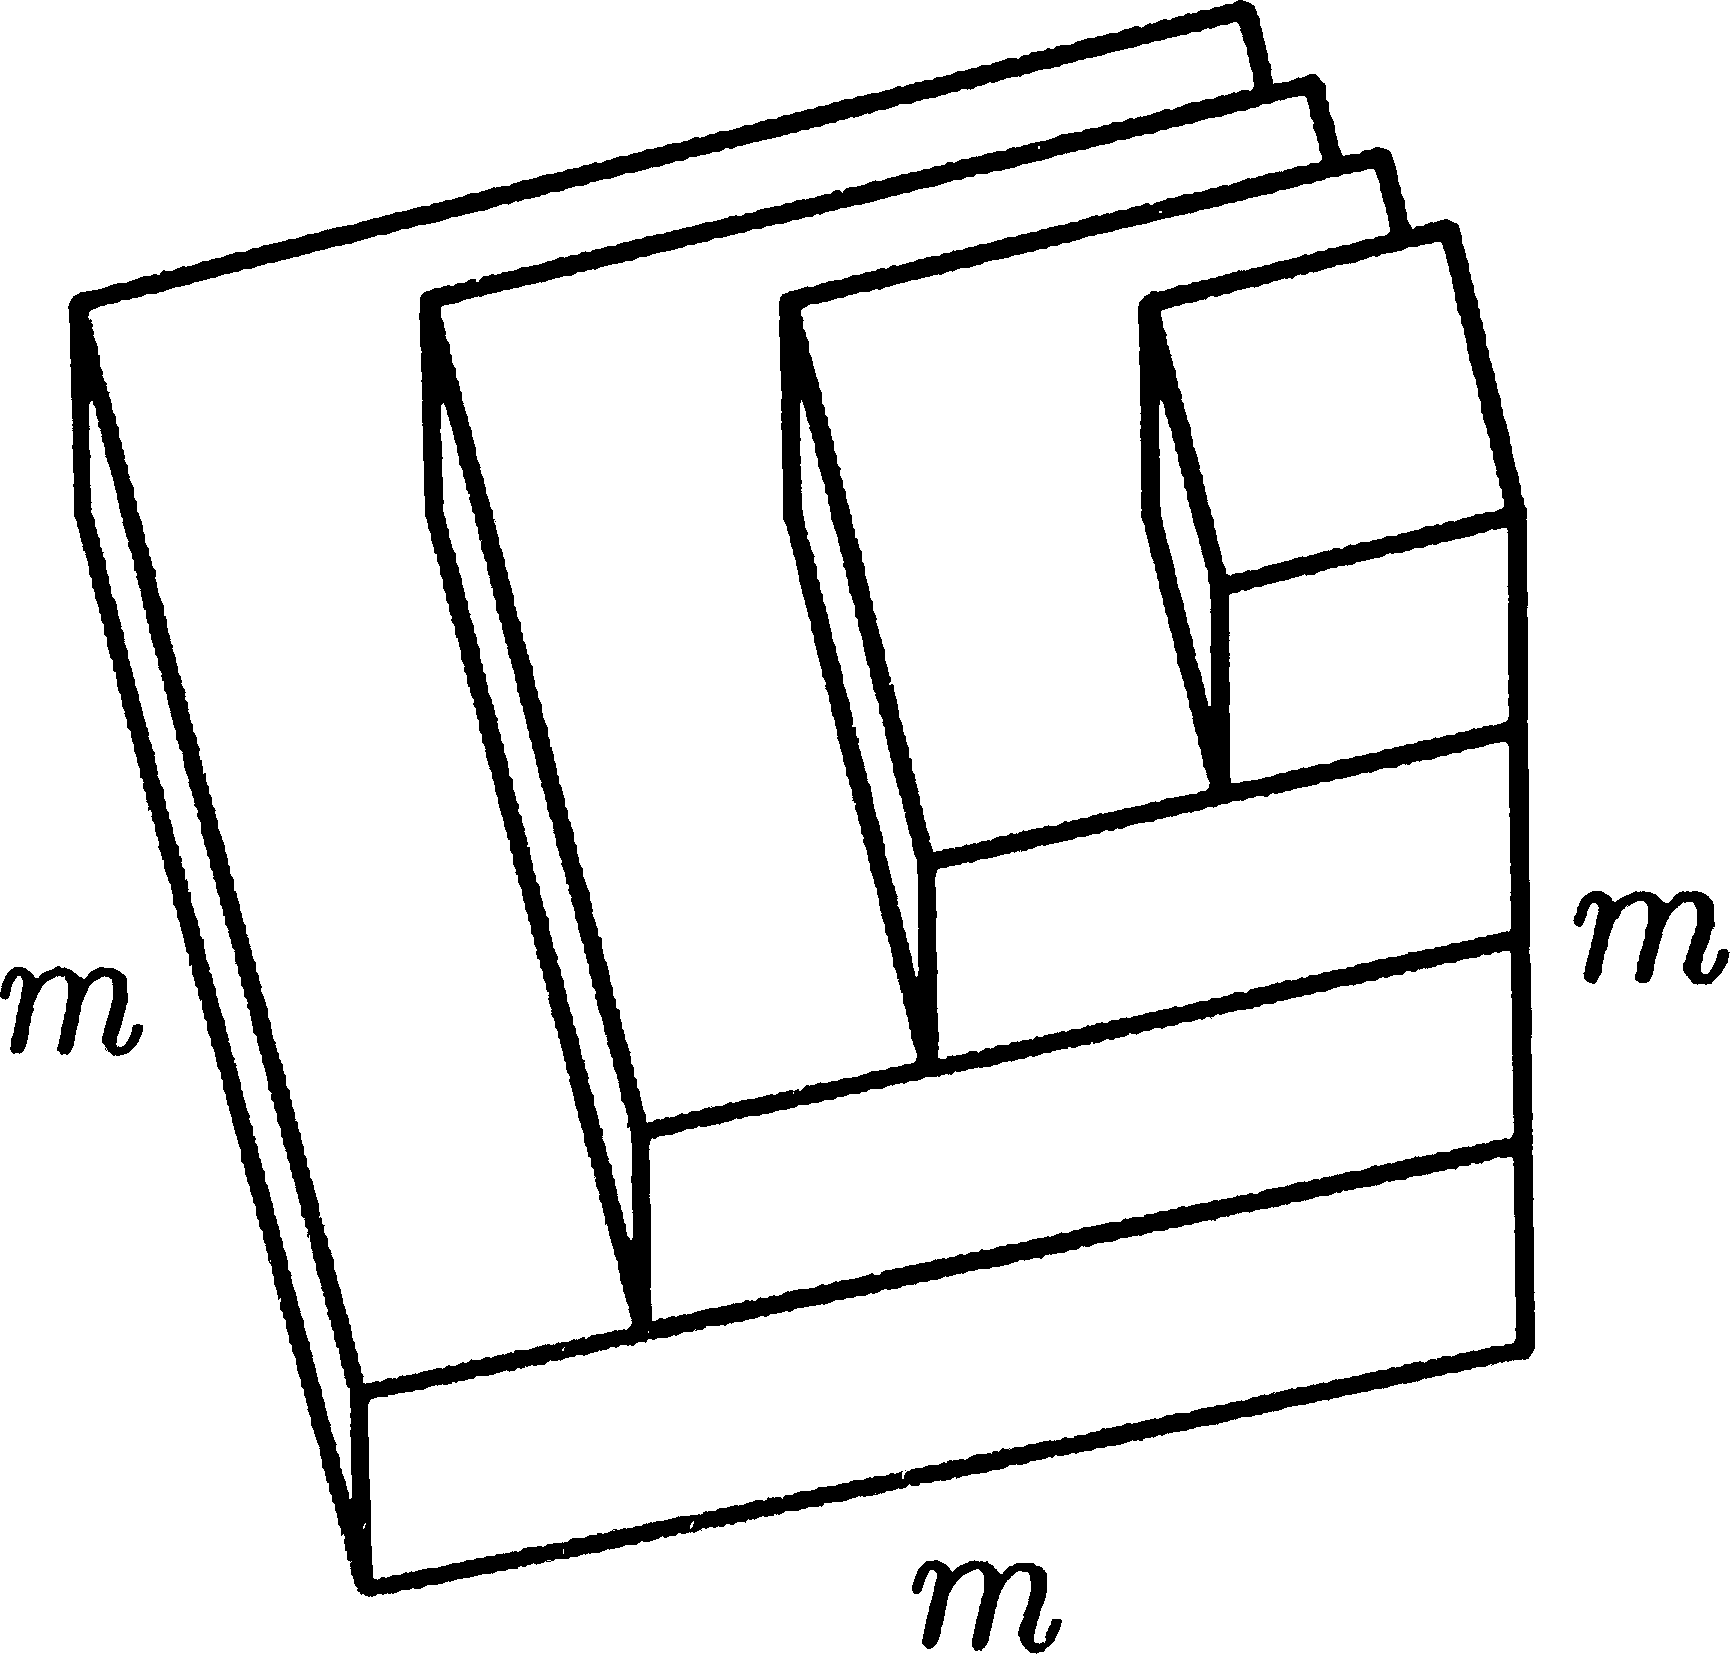
\includegraphics[width=0.2\textwidth]{images/gepyramid.png}

\vspace{-15mm}
\begin{minted}[fontsize=\footnotesize]{python}
def lu(A):
    U, L = A, eye(m,m)
    for k = 0 to m-2:
        for i = k+1 to m-1:
            L[i][k] = U[i][k] / U[k][k]
            for j = k to m-1:
                U[i][j] = U[i][j] - L[i][k] * U[k][j]
    return U, L
\end{minted}

\bigskip
{\scriptsize
\lubullets
}
\end{frame}


\begin{frame}{scaling for solving \textbf{dense} linear systems}

\begin{itemize}
\item the rest of the talk assumes $A\in\RR^{m\times m}$ is square and invertible
\item one \textbf{might} regard the data of ``solve $Ax=b$'' as the matrix $A$ itself
\item then an optimal solver for \textbf{dense} $A$ would require $O(m^2)$ flops
   \begin{itemize}
   \item[$\circ$] one cannot do better because generic dense matrices $A$ have $m^2$ entries, and thus touching each entry is $O(m^2)$
   \end{itemize}
\item however, we know GEBS is $O(m^3)$, thus not optimal
\item $\exists$ solver algorithms\footnote{these ``fast solvers'' can even be stable with respect to rounding errors? this is not clear to me! see J.~Demmel, I.~Dumitriu, O.~Holtz, and R.~Kleinberg (2007). \emph{Fast matrix multiplication is stable}, Numer.~Math.~106 (2), 199--224} for dense $A\in\RR^{m\times m}$ which scale as $O(m^{\,2.376})$
   \begin{itemize}
   \item[$\circ$] famously starting with V.~Strassen (1969). \emph{Gaussian elimination is not optimal}, Numer.~Math.~13, 354--356
   \end{itemize}
\item however, this ``fast dense solver'' game is not practical
   \begin{itemize}
   \item[$\circ$] fascinating algebra, but little impact on scientific/engineering software
   \item<2>[$\circ$] \alert{for the applications of greatest interest, $O(m^{\,2.376})$ is catastophically slow}
   \end{itemize}
\end{itemize}
\end{frame}


\begin{frame}{optimal solvers for $Ax=b$, arising from applications?}

\begin{itemize}
\item \alert{the rest of the talk assumes the size of the data is $m$}
   \begin{itemize}
   \item[$\circ$] $m$ = (number of unknowns) = (number of rows in $A$) = (length of $b$)
   \item[$\circ$] $A\in\RR^{m\times m}$, $b \in \RR^m$
   \end{itemize}
\item are there special classes of matrices $A\in\RR^{m\times m}$, which routinely arise in applications, for which there are $O(m^1)$ solvers?
   \begin{itemize}
   \item[$\circ$] yes
   \end{itemize}
\item $\exists O(m^1)$ solvers $\implies$ $\exists$ exploitable matrix structure
   \begin{itemize}
   \item[$\circ$] these are \emph{not} generic, dense matrices
   \item[$\circ$] most are sparse, but some are dense!
   \end{itemize}
\item a \emph{huge} amount of science/engineering-relevant software supports these special matrix classes and optimal solver algorithms
\end{itemize}
\end{frame}


\section{banded matrices}

\begin{frame}{banded matrices}

\begin{definition}
a square matrix $A$ is \emph{banded} with \emph{lower bandwidth} $p$ and \emph{upper bandwidth} $q$ if
    $$i > j + p \,\,\text{ or }\,\, j > i + q \quad \implies \quad a_{ij} = 0$$
\end{definition}

\begin{itemize}
\item example non-zero pattern

with $p=2,q=4$:

\vspace{-7mm}
\hspace{55mm} 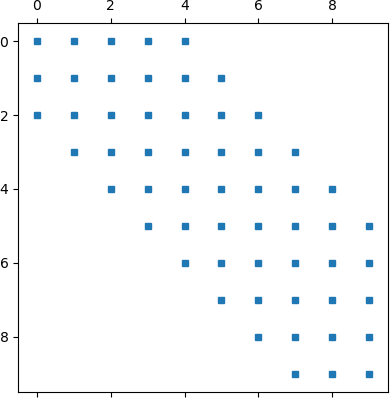
\includegraphics[width=0.28\textwidth]{images/banded.png}

\medskip
\item I have already mentioned tridiagonal matrices

\vspace{-2mm}
\hfill
{\scriptsize $\displaystyle \begin{bmatrix} \bullet & \bullet & & \\ \bullet & \bullet & \bullet & \\ & \bullet & \bullet & \bullet \\ & & \bullet & \bullet \end{bmatrix}$} 

\vspace{-5mm}
   \begin{itemize}
   \item[$\circ$] tridiagonal matrices are banded with $p,q=1,1$
   \end{itemize}
\end{itemize}
\end{frame}


\begin{frame}[fragile]
\frametitle{generating and viewing banded matrices}

\begin{itemize}
\item random $m=10$ matrix with bandwidths $p=2$ (lower) and $q=4$ (upper):

\bigskip
\begin{minted}[fontsize=\footnotesize]{python}
from numpy import tril, triu
from numpy.random import randn
from matplotlib.pyplot import spy, show
m,p,q = 10,2,4
A = tril(triu(randn(m,m),-p),+q)
spy(A,markersize=5.0)
show()
\end{minted}
\end{itemize}

\vspace{-10mm}
\hfill 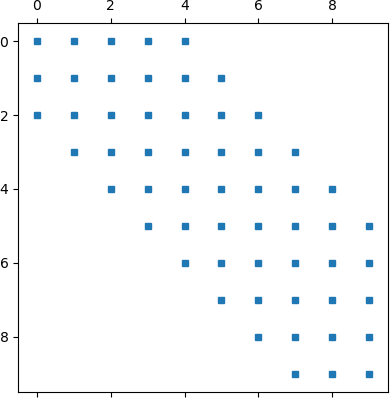
\includegraphics[width=0.38\textwidth]{images/banded.png}
\end{frame}


\begin{frame}[fragile]
\frametitle{banded LU decomposition}

\begin{itemize}
\item specializing LU decomposition to banded matrices is straightforward
\item the version below computes $A=LU$ \emph{without} pivoting
   \begin{itemize}
   \item[$\circ$] skipping pivoting is generally unstable, but o.k.~for nice classes of matrices 
   \item[$\circ$] the algorithm below is \emph{in place}; it overwrites $A$ with $L$ and $U$
   \item[$\circ$] $2pqm + (\text{lower}) = O(pqm) = O(m)$ flops
   \item[$\circ$] the tridiagonal case is often called the \emph{Thomas} algorithm
   \end{itemize}

\medskip
\begin{center}
\begin{minipage}{0.8\textwidth}
\begin{minted}[fontsize=\footnotesize]{python}
def lu_banded(A):
    for k = 0 to m-2:
        for i = k+1 to min{k+p,m}:
            A[i][k] = A[i][k] / U[k][k]
        for j = k+1 to min{k+q,m}:
            for i = k+1 to min{k+p,m}:
                A[i][j] = A[i][j] - A[i][k] * A[k][j]
    return A
\end{minted}
\end{minipage}
\end{center}

\bigskip
\item banded LU is optimal $O(m)$
   \begin{itemize}
   \item[$\circ$] but the constant in ``$O(m)$'' is proportional to the product $pq$ of bandwidths
   \end{itemize}
\end{itemize}
\end{frame}


\begin{frame}{effect of pivoting on banded LU}

\begin{itemize}
\item pivoting expands the band, often acceptably
\item \emph{theorem.} if $A$ is $p,q$ banded then $PA=LU$ where $U$ has upper bandwidth at most $p+q$; though $L$ can have any bandwidth, it has at most $p+1$ nonzeros per column
\end{itemize}


\includegraphics[width=0.25\textwidth]{images/banded-A.png}

\mbox{
\includegraphics[width=0.25\textwidth]{images/banded-PA.png} $=$ 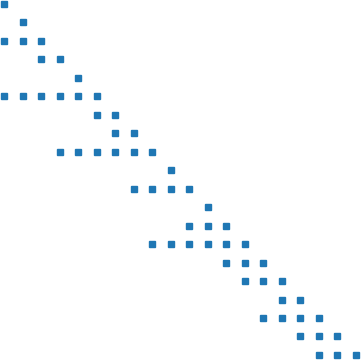
\includegraphics[width=0.25\textwidth]{images/banded-L.png} 
\includegraphics[width=0.25\textwidth]{images/banded-U.png}}

FIXME
\end{frame}


\begin{frame}{where do banded matrices come from?}

\begin{itemize}
\item TWO-POINT BC
\item 2D POISSON FD
\end{itemize}
\end{frame}



\section{circulant matrices}

\begin{frame}{circulant matrices}

\begin{definition}
a square matrix $A \in \RR^{m\times m}$ is \emph{circulant} if each wrapped diagonal is constant, that is, there is a vector $c \in \RR^m$, the first column of $A$, so that
	$$a_{ij} = c_{\,i - j \hspace{-2mm} \mod m}$$
\end{definition}

\begin{itemize}
\item example:
	$$A = \begin{bmatrix} 2 & 7 & -1 & 3 & 8 \\ 8 & 2 & 7 & -1 & 3 \\ 3 & 8 & 2 & 7 & -1 \\ -1 & 3 & 8 & 2 & 7 \\ 7 & -1 & 3 & 8 & 2 \end{bmatrix} \qquad \text{ is from } c = \begin{bmatrix} 2 \\ 8 \\ 3 \\ -1 \\ 7 \end{bmatrix}$$
\item these are \emph{dense} matrices
\item can be stored with $O(m)$ storage \dots store $c$ not $A$
\end{itemize}
\end{frame}


\begin{frame}{downshifting to circulate}

\begin{itemize}
\item let $D_m$ be the \emph{downshift} matrix, for example
{\small
	$$D_5 = \begin{bmatrix} & & & & 1 \\ 1 & & & & \\ & 1 & & & \\ & & 1 & & \\ & & & 1 & \end{bmatrix} \hspace{50mm}$$
}
so that, for example,
{\small
	$$D_5 c = \begin{bmatrix} & & & & 1 \\ 1 & & & & \\ & 1 & & & \\ & & 1 & & \\ & & & 1 & \end{bmatrix} \begin{bmatrix} 2 \\ 8 \\ 3 \\ -1 \\ 7 \end{bmatrix} = \begin{bmatrix} 7 \\ 2 \\ 8 \\ 3 \\ -1 \end{bmatrix} \hspace{45mm}$$
}
\item then, for example: \qquad $\displaystyle A = 2 I + 8 D_5 + 3 D_5^2 + (-1) D_5^3 + 7 D_5^4$

\vspace{-50mm}
{\scriptsize
\hfill $\displaystyle \boxed{\begin{matrix} \text{recall} \\ \\ A = \begin{bmatrix} 2 & 7 & -1 & 3 & 8 \\ 8 & 2 & 7 & -1 & 3 \\ 3 & 8 & 2 & 7 & -1 \\ -1 & 3 & 8 & 2 & 7 \\ 7 & -1 & 3 & 8 & 2 \end{bmatrix} \end{matrix}}$
}

\vspace{30mm}
\item generally, if $A$ is circulant with first column $c$ then
	$$A = c_0 I + c_1 D_m + c_2 D_m^2 + \dots + c_{m-1} D_m^{m-1} = \sum_{k=0}^{m-1} c_k D_m^k$$
\end{itemize}
\end{frame}


\begin{frame}{diagonalization and polynomials}

\begin{itemize}
\item recall that a square matrix $A$ has an \emph{eigenvector} $v$ if $v$ is nonzero and $Av=\lambda v$ for some scalar $\lambda$, in which case $\lambda$ is the \emph{eigenvalue}
\item also recall that if $A$ is $m\times m$, and if there is a set of $m$ linearly-independent eigevectors $v_0,\dots,v_{m-1}$ of $A$, then we say $A$ is \emph{diagonalizable}:
	$$AV = V \Lambda \qquad \iff \qquad A = V \Lambda V^{-1}$$
\item suppose we have a scalar polynomial of degree $n$:
	$$p(\xi) = c_0 + c_1 \xi + c_2 \xi^2 + \dots + c_n \xi^n$$
\item the matrix $p(A)$, for a diagonalizable matrix $A$, is easily computed:
\begin{align*}
p(A) &= c_0 + c_1 A + c_2 A^2 + \dots + c_n A^n \\
     &= c_0 I + c_1 V \Lambda V^{-1} + c_2 \left(V \Lambda V^{-1}\right)^2 + \dots + c_n \left(V \Lambda V^{-1}\right)^n \\
     &= c_0 V I V^{-1} + c_1 V \Lambda V^{-1} + c_2 V \Lambda^2 V^{-1} + \dots + c_n V \Lambda^n V^{-1} \\
     &= V \left(c_0 + c_1 \Lambda + \dots + c_n \Lambda^n\right) V^{-1} = V \begin{bmatrix} p(\lambda_0) & & \\ & \ddots & \\ & & p(\lambda_{m-1}) \end{bmatrix} V^{-1}
\end{align*}
\end{itemize}
\end{frame}


\begin{frame}{y}

\begin{itemize}
\item FIXME we have circulant as poly in $D_m$
\item diagonalize $D_m$ by $F_m$ using $\omega_m$ s.t. $\omega_m^m = 1$
\end{itemize}
\end{frame}


\begin{frame}{y}

\begin{itemize}
\item what is this matrix $F_m$? the DFT
\item the FFT applies $F_m$ in $O(m\log m)$ time, as long as $m$ is ``highly composite''
\item also $F_m^{-1}$
\item if $A$ is circulant, we can solve $Ax=b$ in $O(m\log m)$ time
\end{itemize}
\end{frame}


\section{sparse storage}

\begin{frame}{y}

\begin{itemize}
\item x
\end{itemize}
\end{frame}


\section{paradigm of the 1990s: preconditioned Krylov iterations}

\begin{frame}{y}

\begin{itemize}
\item x
\end{itemize}

\hfill 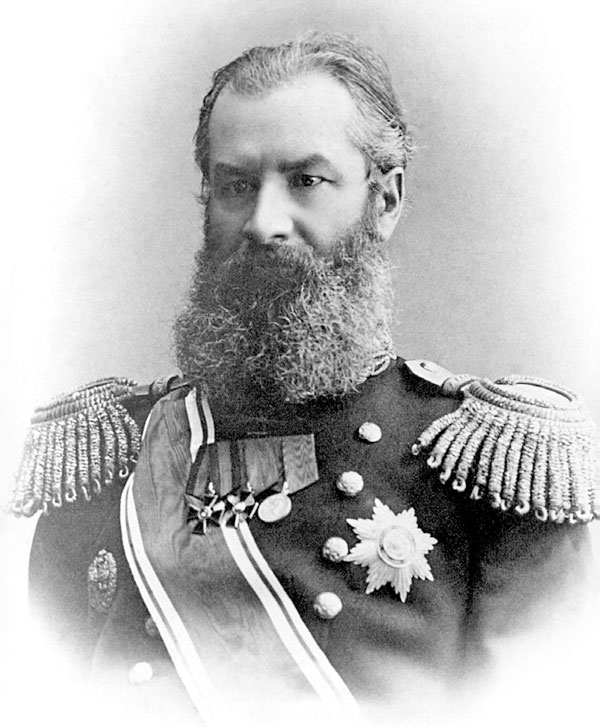
\includegraphics[width=0.2\textwidth]{images/akrylov.jpg}
\end{frame}


\begin{frame}{y}

\begin{itemize}
\item x
\end{itemize}
\end{frame}


\begin{frame}{references}

\begin{columns}
\begin{column}{0.8\textwidth}
\begin{itemize}
{\small
%\item[] \textbf{A.~Brandt (1977)}. \emph{Multi-level adaptive solutions to boundary-value problems}, Mathematics of Computation 31 (138), 333--390
%    \begin{itemize}
%    \item[$\circ$] the guru of multigrid should be better known
%    \end{itemize}
%\item[] \textbf{W.~Briggs, V.~E.~Henson, \& S.~McCormick (2000)}.  \emph{A Multigrid Tutorial}, 2nd ed., SIAM Press, Philadelphia
\item[] \textbf{E.~Bueler (2021)}. \emph{PETSc for Partial Differential Equations}, SIAM Press, Philadelphia
    \begin{itemize}
    \item[$\circ$] Krylov methods, multigrid, optimal PDE solvers
    \end{itemize}
\item[] \textbf{G.~Golub \& C.~van Loan (2013)}. \emph{Matrix Computations}, 4th ed., Johns Hopkins University Press, Baltimore
    \begin{itemize}
    \item[$\circ$] algorithms, banded \& circulant matrices, sparse storage
    \end{itemize}
\item[] \textbf{L.~Trefethen \& D.~Bau (2022)}. \emph{Numerical Linear Algebra}, 25th anniversary ed., SIAM Press, Philadelphia
    \begin{itemize}
    \item[$\circ$] clear thinking on matrices and core algorithms
    \end{itemize}
%\item[] \textbf{U.~Trottenberg, C.~Oosterlee, \& A. Schuller (2001)}.  \emph{Multigrid}, Elsevier, Oxford
}
\end{itemize}
\end{column}
\begin{column}{0.17\textwidth}
%\hfill 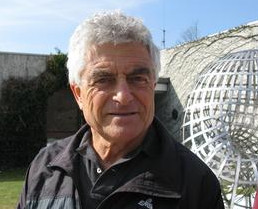
\includegraphics[width=\textwidth]{images/abrandt.jpg}
%\vspace{7mm}
\hfill 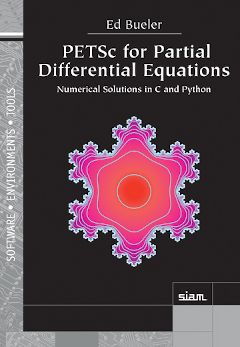
\includegraphics[width=0.8\textwidth]{images/bueler.jpg}

\medskip
\hfill 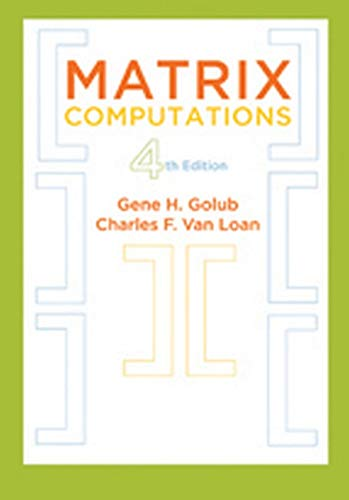
\includegraphics[width=0.8\textwidth]{images/golubvanloan.jpg}

\medskip
\hfill 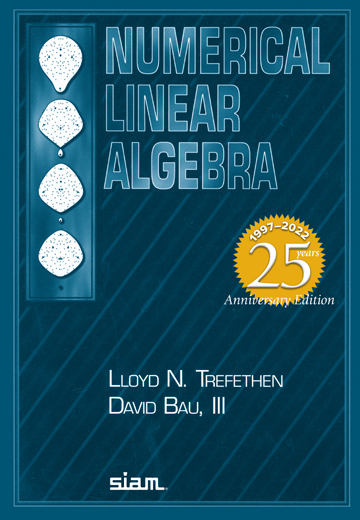
\includegraphics[width=0.8\textwidth]{images/trefethenbau.jpg}
%\vspace{5mm}
\end{column}
\end{columns}
\end{frame}

\end{document}
